\apendice{Especificación de Requisitos}
Un caso de uso puede definirse como una 'secuencia de acciones realizadas por el sistema, que producen un resultado observable y valioso para un usuario en particular'\cite{Cillero2024}. Los diagramas de casos de uso mostrados a continuación ilustran estas acciones del sistema relacionadas con los 3 tipos de usuario contemplados en la presente solución tecnológica: Paciente (persona con Enfermedad de Párkinson), profesional (profesional sanitario) y administrador.
\section{Diagramas de casos de uso}
Con el objetivo de mostrar las mejoras en la aplicación web que se han realizado durante este proyecto y dar también un contexto general del funcionamiento total de la aplicación, se muestran una serie de diagramas de casos de uso.

Las mejoras realizadas en la aplicación web afectan únicamente a los usuarios de tipo 'paciente' y 'profesional'. Debido a ello se muestra en la figura \ref{fig:Casosdeuso} un diagrama de casos de uso relacionado con estos dos tipos de usuarios.
\begin{figure}[h]
    \centering
    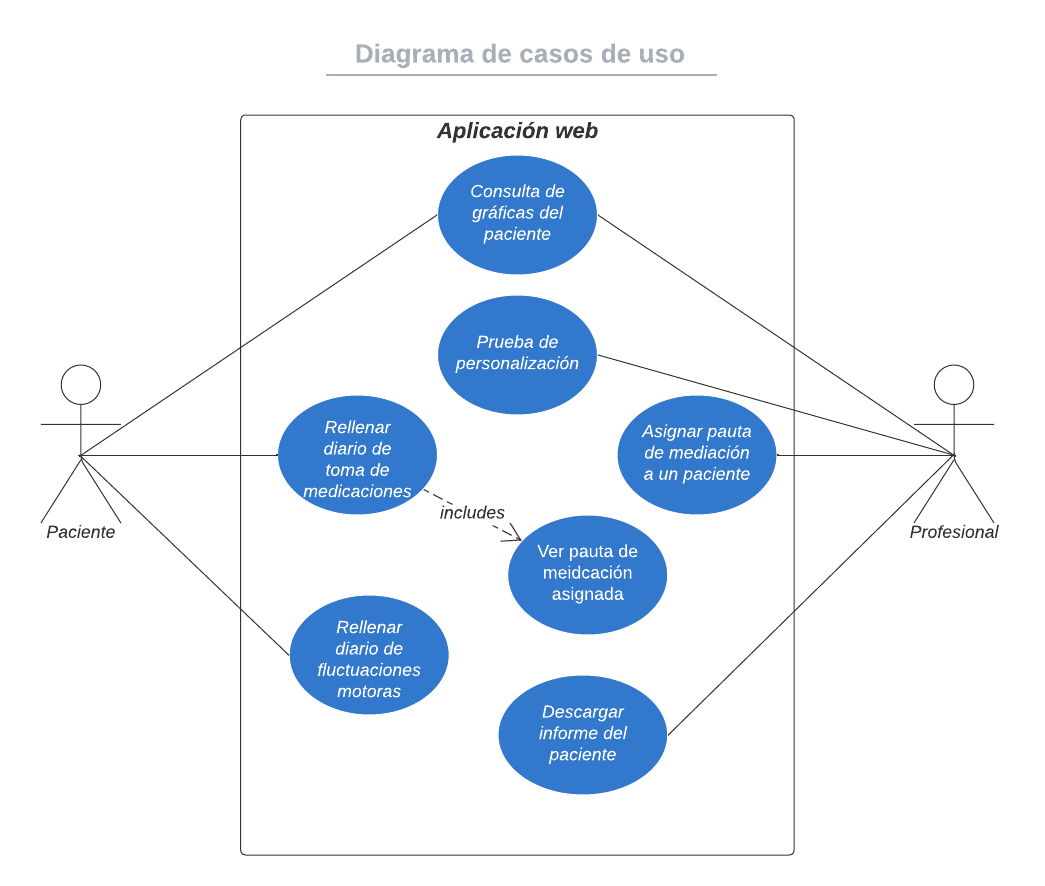
\includegraphics[width=1\textwidth]{img/Casosdeuso.png}
    \caption{Casos de uso de las nuevas funciones de la app}
    \label{fig:Casosdeuso}
\end{figure}

Los casos de uso con las funciones totales comunes para todos los usuarios se  mantienen respecto al TFG \cite{Martos2024}, y se muestran en la figura \ref{fig:Casosusotodos}. Los casos de uso incluyendo las funciones exclusivas para el usuario administrador también permanecen intactas desde el proyecto \cite{Martos2024}, y se muestran en la figura \ref{fig:Casosusoadmin}.

Los casos de uso relativos a las funciones de usuarios de tipo profesional y paciente han sido ampliad0s a partir de los descritas el proyecto \cite{Martos2024}, resultando en el diagrama mostrado en la figura \ref{fig:Casospacienteprof}
\begin{figure}[h]
    \centering
    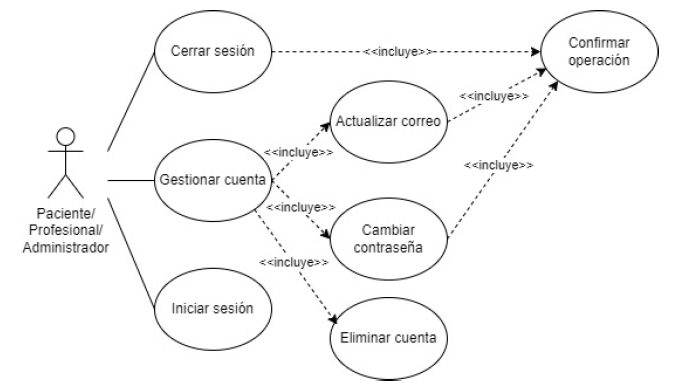
\includegraphics[width=1\textwidth]{img/casosinestodos.png}
    \caption{Casos de uso para todos los usuarios \cite{Martos2024}}
    \label{fig:Casosusotodos}
\end{figure}

\begin{figure}[h]
    \centering
    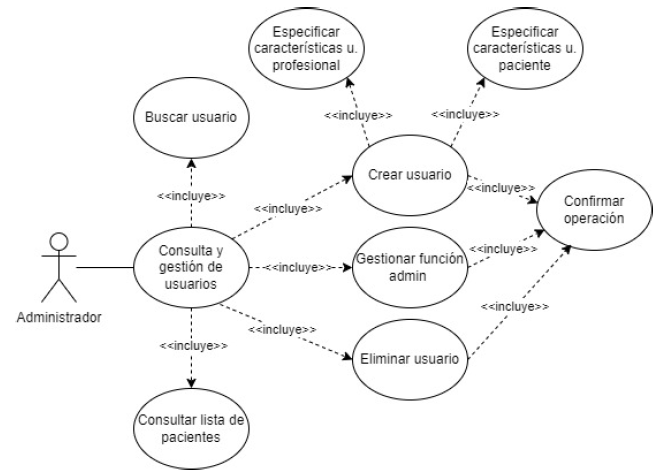
\includegraphics[width=1\textwidth]{img/casosinesadmin.png}
    \caption{Casos de uso para el usuario de tipo 'Administrador' \cite{Martos2024}}
    \label{fig:Casosusoadmin}
\end{figure}

\begin{figure}[h]
    \centering
    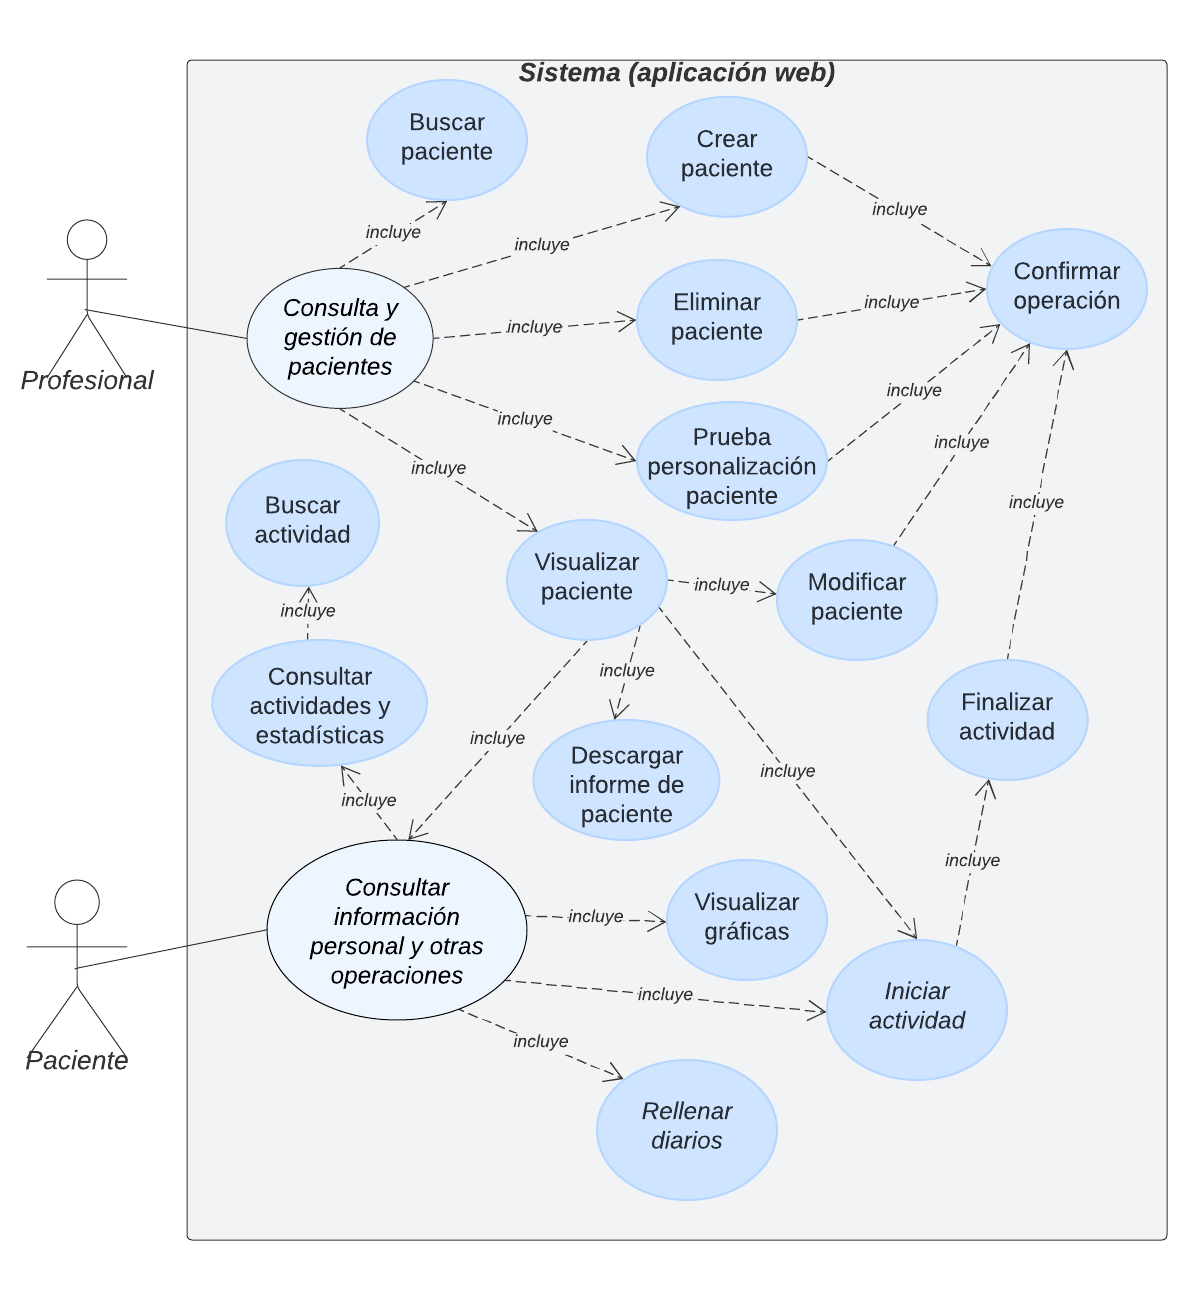
\includegraphics[width=1\textwidth]{img/casospacienteprof.png}
    \caption{Casos de uso para usuarios de tipo 'Profesional' y 'Paciente'. Fuente propia}
    \label{fig:Casospacienteprof}
\end{figure}

\section{Explicación casos de uso.}
Los casos de uso relativos a funcionalidades nuevas de la app, mostrados en la figura \ref{fig:Casosdeuso}, se explican detalladamente en las siguientes tablas: \ref{tab:CU-1}, \ref{tab:CU-2}, \ref{tab:CU-3}, \ref{tab:CU-4}, \ref{tab:CU-5}, \ref{tab:CU-6}
Se puede describir mediante el uso de tablas o mediante lenguaje natural.    

% Caso de Uso 1 -> Consultar Experimentos.
\begin{table}[p]
	\centering
	\begin{tabularx}{\linewidth}{ p{0.21\columnwidth} p{0.71\columnwidth} }
		\toprule
		\textbf{CU-1}    & \textbf{Consulta de gráficas del paciente}\\
		\toprule
		\textbf{Versión}              & 2.0    \\
		\textbf{Autor}                & Carmen Marcos \\
		\textbf{Requisitos asociados} & RF-10 \\
		\textbf{Descripción}          & Acceso por parte del usuario de tipo 'paciente' o 'profesional' a las gráficas creadas a partir de los datos de las actividades registradas por el paciente y los datos de toma de medicaciones y fluctuaciones motoras registrados en los diarios del paciente \\
		\textbf{Precondición}         & El usuario hace click en el botón 'Ver gráficas' situado en la sección de consulta de actividades\\
		\textbf{Acciones}             &
		\begin{enumerate}
			\def\labelenumi{\arabic{enumi}.}
			\tightlist
			\item Se muestran en pantalla los nombres de las gráficas, junto con botones para mostrar/ocultar cada gráfica.
			\item Al pulsar en uno de los botones se muestra la gráfica correspondiente (pueden mostrarse varias gráficas en la pantalla simultáneamente en caso de pulsar varios botones).
                \item Al hacer click una segunda vez en alguno de los botones se ocultará la gráfica correspondiente.
		\end{enumerate}\\
		\textbf{Postcondiciones}        & Para mostrar cada tipo de gráfica de forma adecuada deben cumplirse unas postcondiciones diferentes:
  \begin{enumerate}
        \def\labelenumi{\arabic{enumi}.}
	\tightlist
      \item Gráficas de bloqueos totales y bloqueos por minuto en las actividades: Se requiere que se hayan almacenado datos de actividades previamente
      \item Gráfica de estado del paciente: Deben haber sido registrados en la misma fecha los diarios de toma de medicaciones y de fluctuaciones motoras.
      \item Gráfica de bloqueos por minuto en los diferentes estados (on, off, on con discinesia): Se han registrado datos de actividades y diarios de fluctuaciones motoras en fechas similares
  \end{enumerate}\\
		\textbf{Excepciones}          & Los datos necesaerios para la creación de gráficas no se encuentran almacenados en la base de datos \\
		\textbf{Importancia}          & Media \\
		\bottomrule
	\end{tabularx}
	\caption{CU-1 Consulta de gráficas del paciente.}
        \label{tab:CU-1}
\end{table}

\begin{table}[p]
	\centering
	\begin{tabularx}{\linewidth}{ p{0.21\columnwidth} p{0.71\columnwidth} }
		\toprule
		\textbf{CU-2}    & \textbf{Prueba de personalización}\\
		\toprule
		\textbf{Versión}              & 2.0    \\
		\textbf{Autor}                & Carmen Marcos \\
		\textbf{Requisitos asociados} & RF-08\\
		\textbf{Descripción}          & Prueba diseñada para personalizar los segundos consecutivos de reposo que el sensor MPU-6050 considerará como congelamiento de la marcha. El usuario 'profesional' tiene acceso a la misma, pretendiendo que en una primera cita de explicacion y puesta en marcha de la solución tecnológica pueda asistir al paciente durante la realización de la prueba. 
        %Los resultados de la prueba se guardarán en la tabla 'personalización' de la base de datos. Esta actividad no percibe episodios de congelamiento de la marcha, teniendo como único objetivo obtener una idea significativa de los segundos que tarda el usuario en dar 1 paso, a partir de los cuales se calculará posteriormente mediante una fórmula el número personalizado de segundos. 
        \\
		\textbf{Precondición}         & El profesional hace click en el botón 'consultar' situado en la tabla de pacientes para llegar al apartado de información del paciente correspondiente. Posteriormente, hace click en el botón 'personalización', redirigiéndose a la pantalla de realización de prueba.
		\\
		\textbf{Acciones}             & \begin{enumerate} \def\labelenumi{\arabic{enumi}.}
	\tightlist
		\item Se mostrarán los botones 'iniciar actividad' y 'volver al menú'
        \item Al pulsar el botón 'iniciar actividad' se mostrarán en pantalla los datos (pasos, velocidad, duración), al igual que en una actividad normal.
        \item Al sobrepasar los 10 pasos de actividad, se muestra un botón de 'finalizar actividad'%ya que se considera la actividad realizada una muestra válida para el cálculo del tiempo medio que transcurre en cada paso.
        \item Al pulsar el botón 'finalizar actividad' se mostrará en pantalla el número de segundos personalizado que se ha calculado, así como un mensaje de confirmación que preguntará al usuario si se desean guardar los datos.
        \item En caso afirmativo, se guardarán los datos en la tabla 'personalización' de la base de datos.
		\end{enumerate}\\
		\textbf{Postcondiciones}        & 		El dispositivo se encuentra conectado mediante bluetooth al dispositivo correspondiente. El archivo bridge.py y el servidor node.js están ejecutándose para establecer comunicación bidireccional entre el dispositivo y la página web. %Estos archivos deben haber sido activados ejecutando el primero y escribiendo node server.js en la terminal desde el directorio del segundo.
  \\
		\textbf{Excepciones}          & Los archivos bridge.py y server.js no funcionan adecuadamente o no se establece una conexión bluetooth adecuada con el dispositivo. \\
		\textbf{Importancia}          & Alta \\
		\bottomrule
	\end{tabularx}
	\caption{CU-2 Prueba de personalización.}
        \label{tab:CU-2}
\end{table}

\begin{table}[p]
	\centering
	\begin{tabularx}{\linewidth}{ p{0.21\columnwidth} p{0.71\columnwidth} }
		\toprule
		\textbf{CU-3}    & \textbf{Asignar pauta de medicación a un paciente}\\
		\toprule
		\textbf{Versión}              & 2.0    \\
		\textbf{Autor}                & Carmen Marcos \\
		\textbf{Requisitos asociados} & RF-03 \\
		\textbf{Descripción}          & El usuario de tipo 'profesional' puede asociar a uno de sus pacientes asignados una pauta de medicación, especificando cuantas medicaciones relacionadas con síntomas motores del Párkinson deben tomar diariamente, cuáles y cuántas tomas en cada una.
        \\
		\textbf{Precondición}         & El usuario habrá iniciado sesión en la aplicación web utilizando una cuenta de tipo 'profesional' válida. El usuario pulsa el botón 'agregar pauta', situado en la pantalla de inicio.
		\\
		\textbf{Acciones}             & \begin{enumerate} \def\labelenumi{\arabic{enumi}.}
	\tightlist
		\item El usuario visualiza el formulario a rellenar, seleccionando el paciente para el cual desea agregar una pauta de medicación.
        \item El usuario selecciona el número de medicaciones distintas que deben ser tomadas durante el día. El contenido del formulario se adaptará dinámicamente a este número, mostrando tantos cuadros de medicación como sean necesarios.
        \item El usuario ajusta los nombres de las medicaciones y el número de tomas de cada una de ellas que deben realizarse cada día.
        \item Tras haber completado el formulario, el usuario pulsará el botón "guardar".
        \item Los datos se almacenarán en la tabla 'pautas' de la base de datos
		\end{enumerate}\\
		\textbf{Postcondiciones}        & 		No existen postcondiciones
  \\
		\textbf{Excepciones}          & No existen excepciones \\
		\textbf{Importancia}          & Media \\
		\bottomrule
	\end{tabularx}
	\caption{CU-3 Asignar pauta de medicación a un paciente.}
        \label{tab:CU-3}
\end{table}

\begin{table}[p]
	\centering
	\begin{tabularx}{\linewidth}{ p{0.21\columnwidth} p{0.71\columnwidth} }
		\toprule
		\textbf{CU-4}    & \textbf{Rellenar el diario de tomas de medicaciones}\\
		\toprule
		\textbf{Versión}              & 2.0    \\
		\textbf{Autor}                & Carmen Marcos \\
		\textbf{Requisitos asociados} & RF-09 \\
		\textbf{Descripción}          & El usuario de tipo 'paciente' puede acceder al diario de tomas de medicación de la fecha actual, un formulario en el que se especificarán las medicaciones relacionadas con síntomas motores del Párkinson tomadas a lo largo del día y las horas de toma.
        \\
		\textbf{Precondición}         & El usuario habrá iniciado sesión en la aplicación web utilizando una cuenta de tipo 'paciente' válida
		\\
		\textbf{Acciones}             & \begin{enumerate} \def\labelenumi{\arabic{enumi}.}
	\tightlist
		\item Se mostrará el formulario relativo al diario, mostrando en caso de estar disponible la pauta de medicación asignada por el profesional (número y nombre de medicaciones y número de tomas de cada una) como respuestas predeterminadas.
        \item El usuario selecciona el número de medicaciones distintas que han sido tomadas durante el día. El contenido del formulario se adaptará dinámicamente a este número, mostrando tantos cuadros de medicación como sean necesarios.
        \item El usuario ajusta los nombres de las medicaciones, el número de tomas de cada una de ellas y las horas de toma realizadas ese día.
        \item Tras haber completado el formulario, el usuario pulsará el botón "guardar".
        \item Los datos se almacenarán en la tabla 'diario2' de la base de datos
		\end{enumerate}\\
		\textbf{Postcondiciones}        & 		No existen postcondiciones
  \\
		\textbf{Excepciones}          & No existen excepciones \\
		\textbf{Importancia}          & Alta \\
		\bottomrule
	\end{tabularx}
	\caption{CU-4 Rellenar el diario de tomas de medicación.}
        \label{tab:CU-4}
\end{table}

\begin{table}[p]
	\centering
	\begin{tabularx}{\linewidth}{ p{0.21\columnwidth} p{0.71\columnwidth} }
		\toprule
		\textbf{CU-5}    & \textbf{Rellenar el diario de fluctuaciones motoras}\\
		\toprule
		\textbf{Versión}              & 2.0    \\
		\textbf{Autor}                & Carmen Marcos \\
		\textbf{Requisitos asociados} & RF-09 \\
		\textbf{Descripción}          & El usuario de tipo 'paciente' puede acceder al diario de fluctuaciones motoras de la fecha actual, un formulario en el que se especificarán los estados en que se encuentra el paciente a lo largo del día: ON, OFF, ON con discinesia o durmiendo. Se especificará el estado en intervalos de media hora desde las 7:00 hasta las 00:00.
        \\
		\textbf{Precondición}         & El usuario habrá iniciado sesión en la aplicación web utilizando una cuenta de tipo 'paciente' válida
		\\
		\textbf{Acciones}             & \begin{enumerate} \def\labelenumi{\arabic{enumi}.}
	\tightlist
		\item Se mostrará el formulario relativo al diario, constituido por una tabla que tiene las franjas horarias como filas y los estados como columnas, en que el paciente marcará para cada franja horaria el estado correspondiente haciendo click en la columna adecuada.
        \item Una vez que el usuario haya terminado de rellenar el formulario, pulsará el botón 'guardar'.
        \item Los datos se almacenarán en la tabla 'diario' de la base de datos
		\end{enumerate}\\
		\textbf{Postcondiciones}        & 		No existen postcondiciones, aunque el usuario no rellene todas las filas los datos correspondientes a las filas rellenadas podrán guardarse.
  \\
		\textbf{Excepciones}          & No existen excepciones \\
		\textbf{Importancia}          & Alta \\
		\bottomrule
	\end{tabularx}
	\caption{CU-5 Rellenar el diario de fluctuaciones motoras.}
        \label{tab:CU-5}
\end{table}


\begin{table}[p]
	\centering
	\begin{tabularx}{\linewidth}{ p{0.21\columnwidth} p{0.71\columnwidth} }
		\toprule
		\textbf{CU-6}    & \textbf{Descargar el informe del paciente}\\
		\toprule
		\textbf{Versión}              & 2.0    \\
		\textbf{Autor}                & Carmen Marcos \\
		\textbf{Requisitos asociados} & RF-11\\
		\textbf{Descripción}          & 
        \\
		\textbf{Precondición}         & El usuario habrá iniciado sesión en la aplicación web utilizando una cuenta de tipo 'profesional' válida
		\\
		\textbf{Acciones}             & \begin{enumerate} \def\labelenumi{\arabic{enumi}.}
	\tightlist
		\item Se pulsará en el botón 'Generar informe'
        \item Se seleccionará una de las opciones: con gráficas o sin gráficas
        \item Al pulsar en dicha selección se descargará de manera automática el pdf solicitado.
		\end{enumerate}\\
		\textbf{Postcondiciones}        & Existen datos en la base de datos relativos al paciente y actividades realizadas por el mismo.		
  \\
		\textbf{Excepciones}          & \\
		\textbf{Importancia}          & Baja \\
		\bottomrule
	\end{tabularx}
	\caption{CU-6 Descargar informe del paciente.}
        \label{tab:CU-6}
\end{table}
\section{Prototipos de interfaz o interacción con el proyecto.}

\begin{figure}[h]
    \centering
    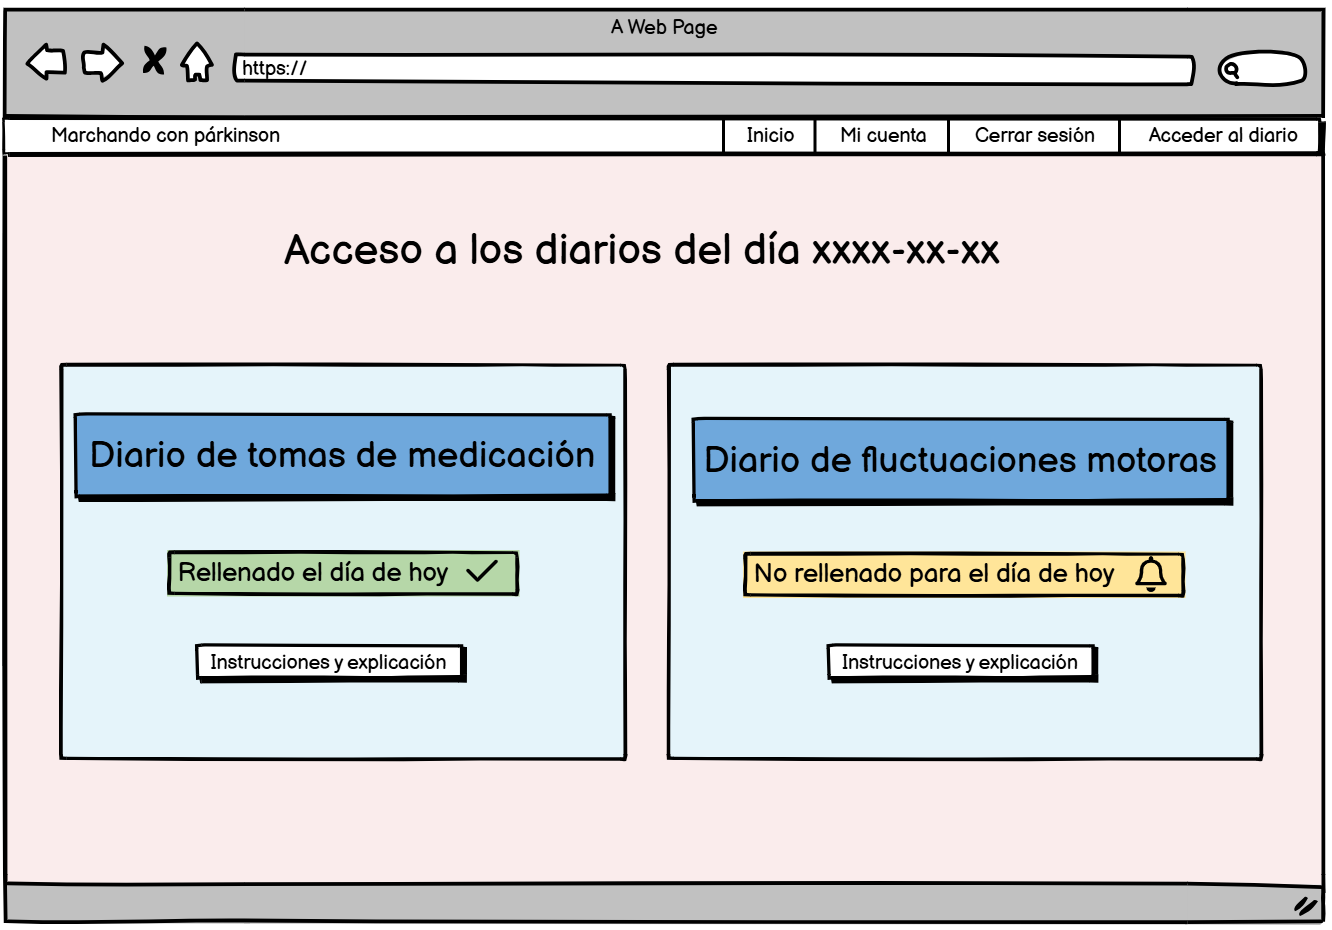
\includegraphics[width=1\textwidth]{img/wdiarios.png}
    \caption{Prototipo de interfaz para el acceso a diarios}
    \label{fig:Wireframediarios}
\end{figure}

\begin{figure}[h]
    \centering
    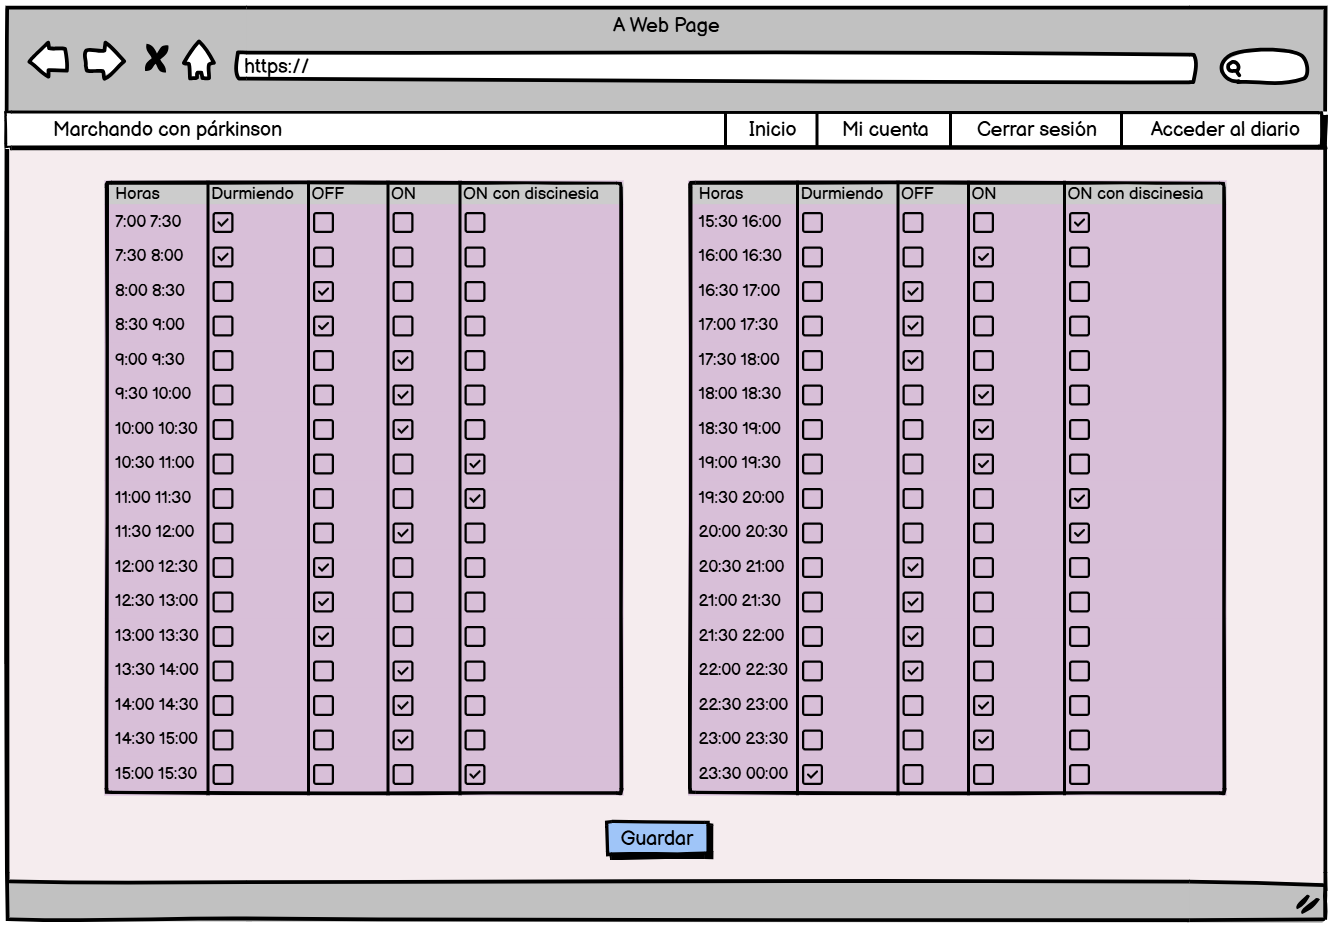
\includegraphics[width=1\textwidth]{img/wdiarioestados.png}
    \caption{Prototipo de interfaz para el diario de fluctuaciones motoras}
    \label{fig:Wireframeestados}
\end{figure}

\begin{figure}[h]
    \centering
    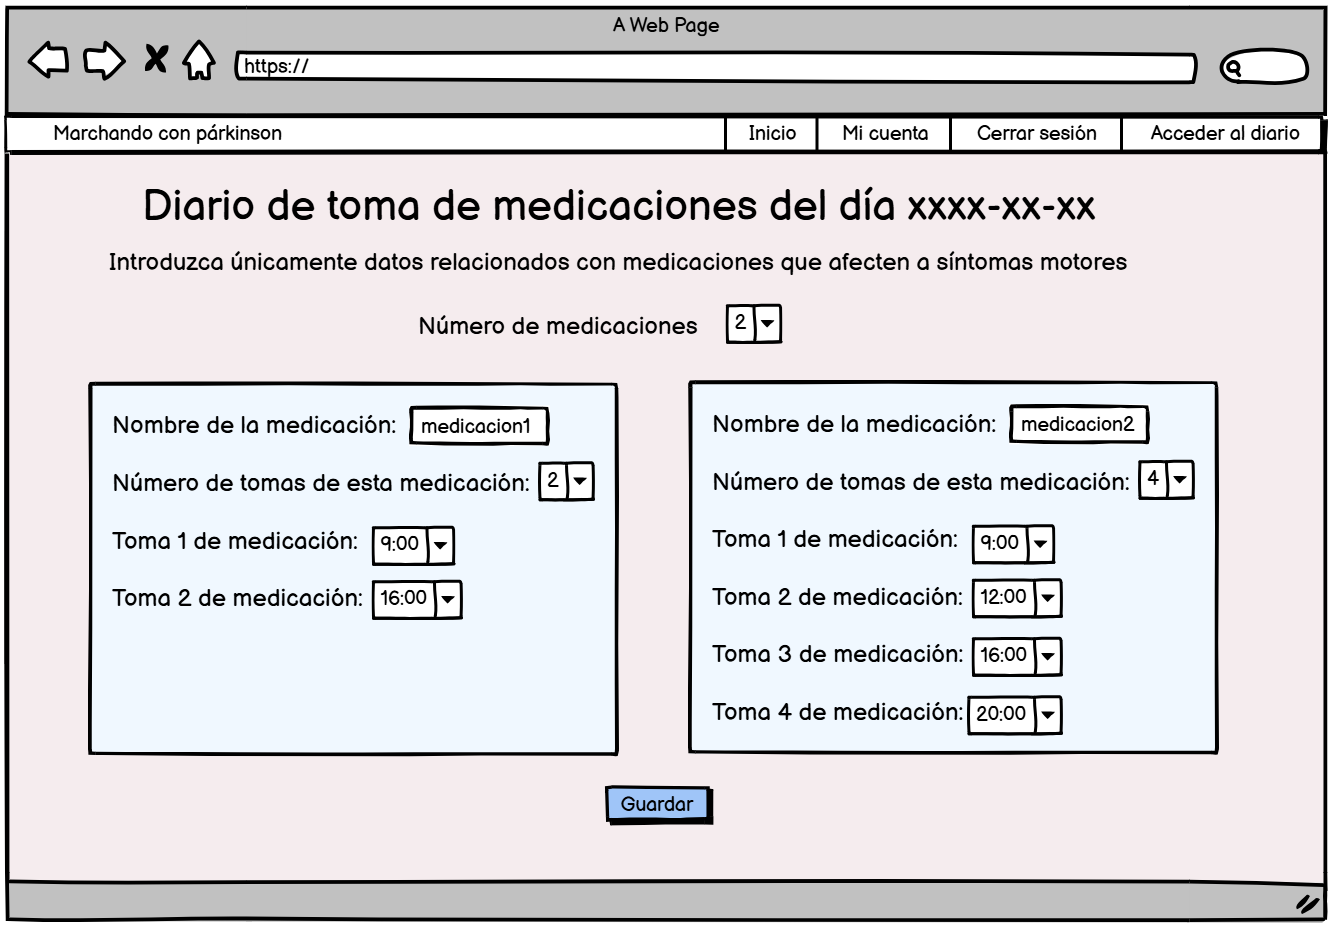
\includegraphics[width=1\textwidth]{img/wdiariotomas.png}
    \caption{Prototipo de interfaz para el diario de toma de medicaciones}
    \label{fig:Wireframemed}
\end{figure}

\begin{figure}[h]
    \centering
    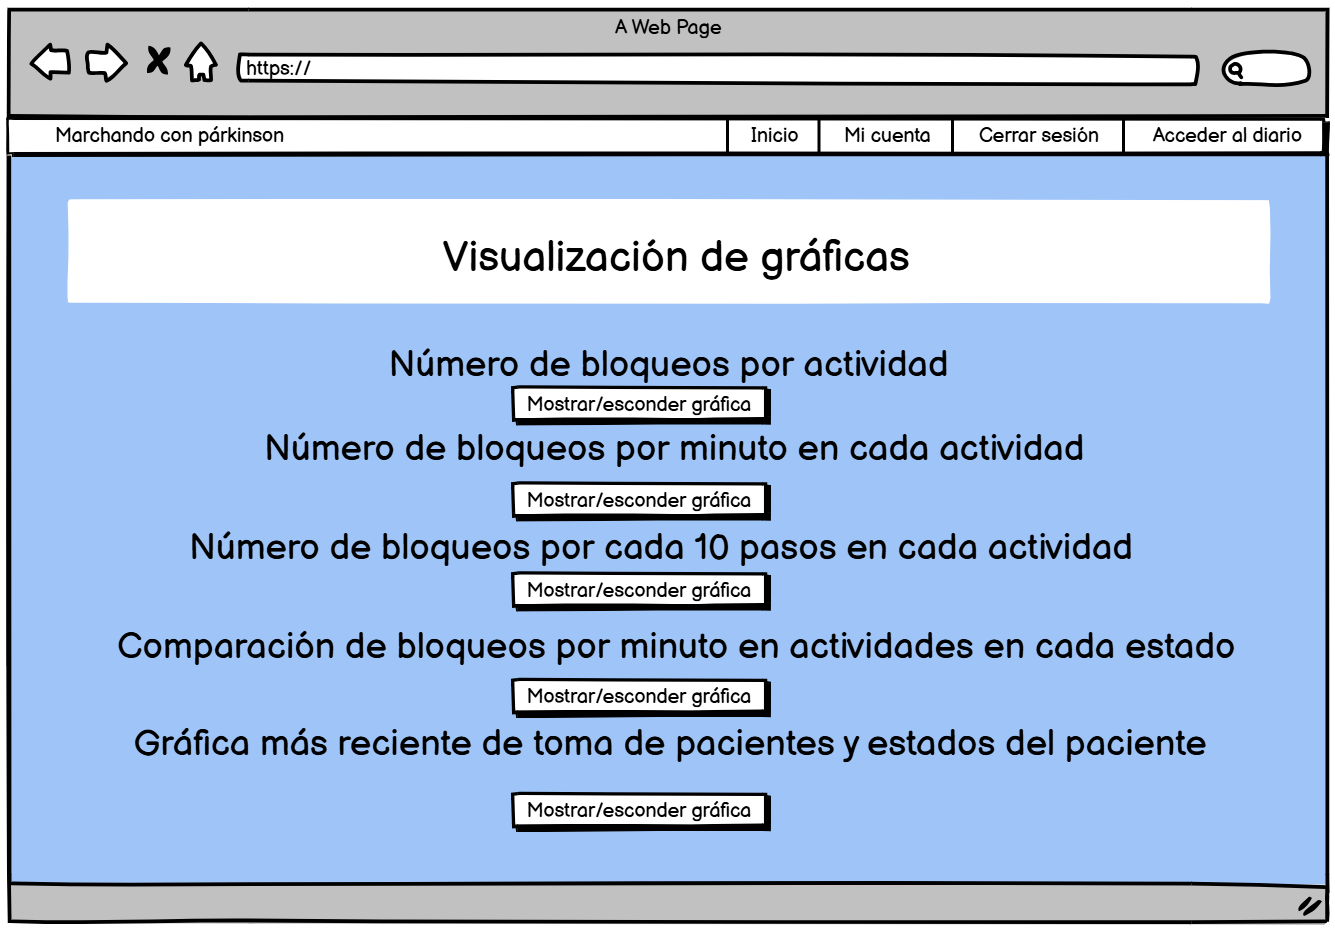
\includegraphics[width=1\textwidth]{img/wgraficas.png}
    \caption{Prototipo de interfaz para la visualización de gráficas}
    \label{fig:Wireframegraficas}
\end{figure}
